%--------------------------------------------------------------------------------------------------
%------------------------------------------------- Chapter --------------------------------------------------------

\chapter{Dispositivo Hipermedial Dinámico: Marco General} \label{cap:2}
\pagenumbering{arabic}

\section{Introducción}
aa
Este capítulo está destina como introducción al marco general de una teoría
que fundamenta el vínculo multidisciplinario para la conceptualización de
una solución que determina funcionalidades mediadas por tecnología de la
información y comunicación (TICs). Se presentarán casos donde se exceden los
niveles de abstracciones y representaciones que el paradigma computacional pueda
abarcar. 

A continuación se comienza con un reconto sobre la inicialización de la
noción de Dispositipvo Hipermedial Dinámico teniendo en cuenta el contexto en
el que se inicia la idea, las distintas actividades y el recorridos que
permitieron su consolidación. Además, al final del capítulo (sección 
\ref{requerimientosdhd}) se establecen nociones básicas sobre aquellos
requerimientos que devienen de los aspectos funcionales del DHD abordados a
través de una propuesta tecnológica incompleta en virtud de las
limitaciones computacionales y tecnológica actualmente disponible. 

Se inicia entonces con la exposición sobre el marco contextual para una
caracterización de los DHD que permitan una primera aproximación hacia la
interpretación necesaria de requerimientos que lo significan. 

El Programa de Investigación, Desarrollo y Transferencia
“Dispositivos Hipermediales Dinámicos” –\url{http://www.mesadearena.edu.ar}-
(CIFASIS: CONICET-UNR-UPCAM), desarrolla desde el 2008 tareas de I+D+T \footnote
{Proyecto Obra Abierta: Dispositivos Hipermediales Dinámicos para educar e
investigar”. Res. CS. – UNR N° 945/2008 Con Subsidio UNR 2008, Res. CS.
N°791/2009 y Subsidio PIP 2009-2011 CONICET N° 0718.}, engloba todas las
actividades, experiencias y resultados logrados sobre la concepción de los DHD.
Existen diferentes proyectos de investigación relacionados donde se vinculan,
entre otros, los principales planos que componen el DHD. Cada uno de estos fijan
elementos que permiten analizar al DHD desde diferentes perspectivas a partir de
tres campos distintos de observación. 

\subsection{El plano de las interacciones del DHD} \label{interacciones}

El plano 1 es abordado en la tesis doctoral "\textit{El Modo Interactivo Del
Dispositivo Hipermedial Dinámico}". Doctorando: Ps. Griselda Guarnieri,
directora: Dra. Patricia San Martín. A continuación se expone algunos de los
conceptos relevante para el espacio de hiperplanos que conforma la dimensión
del DHD.

El problema de investigación que se presenta se centra en el estudio de las
interacciones que se suscitan en la trama compleja que se configura cuando los
sujetos estamos mediados/mediatizados en nuestra comunicación y producción por
las actuales posibilidades de las Tecnologías de la Información y Comunicación
(TIC´s). 

El estudio de las \textbf{interacciones} a través de sus definiciones,
 \textit{caracterización}, \textit{contextualización}, \textit{medición} y
\textit{análisis}. Cada uno de estos elementos estables las referencias de
contactos con otros hiperplanos y proveerán parte de las restricciones y
requisitos que conforman los RequerimientosDHD.

\subsubsection{Las interacciones} \label{relaciones}

Existe una primera concepción de la interactividad que se basaba principalmente
en el análisis de la relación entre el individuo y la computadora. Esta
concepción no estaba fuera de lugar antes del advenimiento de internet,
un ejemplo perfecto de esto es la época donde se jugaba en soledad con la
computadora. Actualmente es extraño que alguien lo haga de esta forma,
generalmente, las actividades lúdicas se realizan en red. Más allá de
entrenamientos o capacitaciones específicas con sistemas expertos y de
simulación con altos grados de automatizaciones que también hoy pueden estar en
red, cuando hablamos de interacción bajo perspectivas constructivistas del
conocimiento, somos sujetos dialógicas constructores de contenidos, que
despliegan sus capacidades críticas en el propio acto responsable.

Existen autores que han tenido en cuenta opciones más amplias para
definir la interactividad y consideran que esta no se agota a la relación
individuo-computadora, sino que implica también al vínculo mediado entre los
individuos.

\begin{defi} [Interactividad]
Retomaremos una definición de interactividad como la capacidad gradual y
variable que tiene un medio de comunicación para darle a los usuarios/lectores
un mayor poder tanto en la selección de contenidos (interactividad selectiva)
como en las posibilidades de expresión y comunicación(interactividad
comunicativa) \cite{lxxiv}.
\end{defi} 


Este autor divide los tipos de interactividad en selectiva comunicativa. La
interactividad selectiva está vinculada principalmente a las posibilidades de
selección de contenidos. A diferencia de la interactividad selectiva, la
comunicativa se basa en que el usuario participe de intercambios dialógicos. “En
la interactividad selectiva, hay un individuo que pregunta o elige una opción y
el sistema le responde automáticamente; en la interactividad comunicativa, hay
un individuo emisor y otro receptor que pueden intercambiar roles. En el primer
caso, el número de posibilidades que tiene el sistema de responder es -por lo
menos en la mayoría de los casos limitado o a veces de una única manera;
mientras que en la segunda opción, la interacción es imprevisible, es decir las
posibilidades de respuesta son infinitas por las características humanas de los
interactuantes” \cite{lxxiv}.

Rost considera, como nosotros nos hemos planteado, que la interactividad
comunicativa es mucho más difícil de cuantificar y medir que la interactividad
selectiva.

Silva \cite{lxxvi} considera que el término interactividad está divido entre los
autores que consideran sólo la relación individuo-máquina y los que creen que es
la relación individuo-individuo mediada por la telemática. Este autor considera
que la interactividad se basa en un plus comunicacional y
quetienetresfundamentos básicos la participación-intervención,
la bidireccionalidad  hidridación y la potencialidad-permutabilidad.

Nuestra postura se ubica con los autores que consideran la interactividad
con un vínculo intersubjetivo mediado por tecnologías, los otros conceptos
generan hoy un reduccionismo innecesario, sobre todo en el campo de la
educación objeto de nuestro estudio.

A su vez, es relevante observar que la interacción entre sujetos no se
puede separar de la comunicación y de la reciprocidad. Nuestra propuesta
considera que ambos términos están interrelacionados, y que la interactividad
integra cuestiones propias del actual contexto físico-virtual visto como red
socio-técnica.

El término interactividad está profundamente entramado con la
digitalización, tanto de información, como de contenidos, no se puede pensar
la interactividad separada de las posibilidades de intercambiar, modificar y
transmitir paquetes de información on line.

La interactividad, a su vez, se separa definitivamente de los dispositivos
transmisivos (unidireccionales), generando intercambios bidireccionales o
multidireccionales. Son innegables las posibilidades que ofrecen las TIC, pero
es necesario un profundo proceso de capacitación y resignificación de las
especificidades de su implementación y esa tarea es aún más compleja que la
creación de más y mejores sistemas tecnológicos.


Las construcciones hipermediales y sus modos de organización son muy
diversos según la epistemología del dominio en el que se inscriban. Pero su
especificidad estructural está en la ausencia de un orden jerárquico que fije
previamente el dominio de su lectura y en la invención de nuevas formas.


La ausencia de interactividad no siempre está ligada a factores
tecnológicos, sino a factores tales como el aspecto relacional, el diseño
conceptual del espacio virtual, tecnología insuficiente, etc.


Es necesario interrogarse, en el caso de las tecnologías informáticas, que
poseen todos los elementos para posibilitar un intercambio interactivo, si este
realmente se realiza. Durante el trayecto de investigación de la tesis
circunscrita al estudio del plano 1, se efectuaron análisis de diversas
implementaciones de educación mediatizada a través de internet, se ha
observado frecuentemente este formato, se reemplaza el texto
impreso en papel por el digital, la fotocopiadora por el texto online, pero no
hay verdaderos canales que posibiliten la interactividad entre los usuarios.

Los espacios virtuales son herramientas válidas, pero es indispensable
considerarlos en toda su potencialidad y especificidad, los mismos pueden
reemplazar viejos modelos, pero sus posibilidades no se agotan allí. Deben ser
utilizados en su dimensión transformadora que solicitan los procesos de
interacción que integran las TIC.

\begin{defi} [Interactividad] En resumen, conceptualizamos la interactividad
como un vínculo intersubjetivo mediado por las TIC que posibilitan el
intercambio bidireccional o multidireccional de mensajes y el intercambio
colaborativo.
\end{defi} 


\begin{figure}
\begin{center}
 \includegraphics[width=4 in,totalheight=3 in] {DHD/hiperplanosDHD}
 % .: 0x0 pixel, 0dpi, 0.00x0.00 cm, bb=
\caption{Hiperplanos del los RequerimientosDHD} \label{hiperplanos}
\end{center}
\end{figure}


\subsection{El plano de los aspectos sistémico del DHD}

El plano 2 es abordado en la tesis doctoral "\textit{La Teoría De Los Sistemas
Complejos Aplicada Al Modelado Del Dispositivo Hipermedial Dinámico}".
Doctorando: Ing. Guillermo Rodriguez, directora: Dra. Patricia San Martín. 

Los primeros trabajos originales fueron en torno a la selección de una teoría de
modelado que contemplara la necesidad de la evaluación de las interacciones como
eventos diferentes en una base de tiempo continuo. La selección del formalismo
DEVS (Discrete EVent dynamics System) aporta una teoría específica que
conjuga ambas necesidades. A su vez, todo el trabajo sobre el desarrollo de
métricas cuali-cuantitativas es también original. La confección de la métrica
fue realizado en conjunto con el equipo de trabajo y aparece reflejado en las
tres tesis que sustentan cada uno de los planos. 

Entonces, del estudio sistémico del DHD se desprende que a través del
\textit{modelados}, la \textit{simulación} y el \textit{análisis} es  posible
describir aspectos importantes de su conceptualización en virtud de sus
dinamismo sistémico.


\subsubsection{Dinamismo sistémico de los DHD}


Una de las ventajas más destacables de las tecnologías actuales con
respecto a otras modalidades a distancia mediadas por el modo transmisión es
la posibilidad de una mayor interacción entre todos los actores del sistema.
Esto facilita cualitativamente la posibilidad de plantear el trabajo
colaborativo y la participación en tiempo sincrónico y asincrónico en las
diversas modalidades de gestión, producción, investigación, desarrollo o
didáctica.


Particularmente los sistemas hipermediales adaptativos tienen como
objetivo construir un espacio capaz de ajustarse a las particularidades de cada
actor, con lo que constituyen una forma única de interacción y reciprocidad
entre el sujeto. Su naturaleza permite configurar entornos para conseguir que
los participantes alcancen los objetivos establecidos mediante contenidos y
recorridos adecuados a sus aptitudes, intereses y preferencias.
Por lo tanto, estos sistemas buscan que el contexto se adapte al usuario y
no al contrario, como sucede en los hipermediales “clásicos”, los cuales
muestran el mismo contenido y los mismos enlaces a todos los usuarios. En
este sentido, para que sea adaptativo debe ser configurado en un entorno
hipermedial y que a su vez, el usuario sea capaz de realizar dicha adaptación
\cite{lxxviii}.


Existe diferencia entre estos sistemas hipermediales adaptativos y un
sistema adaptable ya que éste último se enfoca, básicamente, en proporcionar
al usuario herramientas para la personalización del sistema (color, tipo de
letra, tamaño de letra, etc.), o en contar con interfaces para diferentes
niveles (por ejemplo, experto, principiante, etc.). De este modo, la gran
diferencia es que en un sistema adaptable, el usuario diseña su entorno
seleccionando según sus necesidades o intereses, mientras que un sistema
hipermedial adaptativo emplea un modelo de usuario para proveer adaptación
automática. Aunque también estos últimos pueden contar con características
adaptables \cite{lxxviii}.

De modo general, se define a los sistemas hipermediales adaptativos
como sistemas hipermediales que permiten personalizarse (adaptarse) en
función de los usuario individuales. De este modo, el modelo se desarrolla a
partir de las metas, preferencias, características personales y conocimientos de
cada usuario, el cual lo utilizará y modificará según vaya interactuando con el
sistema y así adecuando la información (contenidos) y los links para la
navegación, a sus necesidades, ya que considera que los usuarios aumentan y
varían sus conocimientos permanentemente. Todo sistema a su vez, refiere a un
contexto, por lo que cabe aclarar que por “contexto” se entiende según Dey
a  ``cualquier información que puede usarse para caracterizar la situación de
una entidad. Entendiendo a la entidad como una persona, lugar u objeto
que es considerado relevante para la interacción entre un usuario y una
aplicación, incluyendo al usuario mismo y la aplicación`` \cite{lxxix}.

De este modo, el contexto es información, y según como se selecciona, procesa y
produce la misma a través de dichos sistemas, se posibilita la adecuación del
mismo con las utilidades para el usuario. Dourish sostiene al respecto que según
la variable situación contextual en la cual la tecnología es utilizada, se
necesita comprender más sobre la relación entre la tecnología informática y el
contexto en la que se encuentra.

El problema del contexto no refiere a cómo lo represento sino que tiene
que ver con un problema de relaciones, es decir, con qué se vincula la
actividad que se desarrolla, de las características del contexto en que se
desenvuelve y a su vez, cómo y porqué las personas que interactúan pueden
tener una comprensión mutua del contexto para sus acciones. La idea de
contexto consiste en un conjunto de características del mismo que rodean las
actividades que se realizan, y que estas características pueden ser codificadas
y hacer viable, de este modo, un sistema de software. Entonces, el contexto no
es algo que permite describir un escenario, sino que es lo que las personas
hacen. Es un producto de la relación, mas que una premisa. Así el contexto y la
actividad no pueden separarse. El contexto no es algo estable, dado, como una
descripción externa a la actividad misma. Por el contrario, aparece y es
sostenido por la misma actividad.

En síntesis, en el marco de este trabajo, los dispositivos hipermediales
dinámicos deben ser sensibles o adaptables al contexto para posibilitar el
dinamismo propio de las interacciones en las comunidades de práctica.


\subsection{El plano de la Ingeniería Computacional de los DHD} \label{plano3}

El plano 3 (figura \ref{hiperplanos}) conforma la base tecnológica y
computacional del DHD, establecida por la arquitectura, el diseño y la
tecnología utilizada para el desarrollo. Estos tres elementos envuelven las
resoluciones funcionales de los requerimientosDHD, en los cuales se sostienen el
grado de concretización de la difinición de DHD. De esta manera se deja
establecido para el resto de la tesis la noción de que cuando hablamos de
Dispositivo Hipermedial Dinámico se hace referencia a los requerimientos
funcionales, computacionales y de diseño; y no necesariamente a su definición
conceptual (\ref{definiciondhd}).

Ahora sí, se comienza con el recorrido hacia la definición conceptual del DHD
mediante las tareas de investigación llevada adelante por el grupo de
investigación Obra Abierta. Los investigadores convocados cuentan con
antecedentes en el estudio de problemáticas vinculadas a la integración efectiva
de las TIC, en diferentes contextos organizacionales educativos tanto públicos
como empresariales (San Martín et al, 2008) fundamentándose en conceptos, método
y bases epistemológicas de la investigación interdisciplinaria en el marco de
los sistemas complejos (García, 2007).

Estos fundamentos posibilitaron, en la continuidad de los distintos proyectos,
la construcción de la noción de Dispositivo Hipermedial Dinámico (DHD) y la
conformación del mencionado programa de investigación que tiene por objetivo
general consolidar el marco teórico, metodológico y de desarrollo tecnológico
del DHD.

En este sentido, el abordaje de las problemáticas se realiza implementando una
metodología de investigación interdisciplinaria que estudia el mismo como
sistema complejo.

\begin{quote} \label{definiciondhd}

Conceptualizamos como Dispositivo Hipermedial Dinámico -DHD- a una red
heterogénea conformada por la conjunción de tecnologías y aspectos sociales que
posibilitan a los sujetos realizar con el otro acciones en interacción
responsable para \textit{investigar}, \textit{aprender}, \textit{dialogar},
\textit{confrontar}, \textit{componer}, \textit{evaluar}, diseminar bajo la
modalidad de taller físico-virtual, utilizando la potencialidad comunicacional,
transformadora y abierta de las TIC, regulados según el caso, por una
“coordinación de contratos”. (Sán Martín, et. al.)
\end{quote} 

Construir una red sociotécnica en un contexto físico virtual con
“presencialidad” subjetiva es sentir la Presencia del otro que cobra sentido
en el compromiso de participación responsable para enseñar y aprender,
investigar y/o   producir  cualquiera    sea   el   grado    y   tecnología
de mediatización. Presencia que en su dimensión simbólica posibilita el vínculo 
intersubjetivo y da lugar a la distancia necesaria para la interrogación,
la representación como “juego al pensamiento” (Enaudeau, 1999), la mediación de
los  discursos (Lasch, 2005) y la acción (Bruner, 2001).

La no presencia se define entonces, como la paradoja de ausencia de sí mismo
en el propio cuerpo, cuerpo que en tanto objeto solitario puede violentarse sin
límite (Olmos: 2006), cuerpo objeto sin distancia, fusionado a otros
objetos(“ser con” en vez de “ser para”), transformado, multiplicado, fragmentado
y “publicitado” en numerosas “redes sociales”, posible de ser “llenado”,
“instrumentalizado”, “editado”, “compactado”...

La utilización o no de TIC en un determinado proceso educativo, investigativo
o de producción y el grado de mediación/mediatización de dicho proceso no puede 
ignorar el contexto del siglo XXI, que da muestra de los múltiples impactos de
la globalización. El problema relevante en una sociedad donde la interactividad
digital es un hecho consumado, no se centra en continuar discutiendo sobre  la
catalogación  de  nuevas nominaciones (e-educación, e-gobierno, e-investigación,
e-comercio, etc.) sino en interrogarnos sobre cómo sostener la presencialidad
subjetiva y la participación ciudadana  responsable e inclusiva. Estas  
dimensiones, pensadas como indisociables, podrían posibilitar quizás la
reflexión sobre la construcción de nuevos vínculos generadores de “civitas”
(Borja, 2006) más allá del grado de mediación/mediatización. Entonces,
observamos que la problemática así planteada excede el tradicional dualismo
presencial - a distancia y lo meramente cuantitativo del grado de mediatización,
centrándose el debate en su real dimensión política dada la emergencia de nuevas
formas culturales físico-virtuales de gestión, transmisión, producción y acceso
-o no- a la información y conocimiento. Esto involucra de hecho las
posibilidades de desarrollo tecnológico colaborativo y la extensiva utilización
abierta de herramientas digitales aptas para múltiples propósitos.

Partiendo de estos posicionamientos, abordaremos a continuación aspectos   
referidos   a    las  condiciones    necesarias   para   el  que hacer
interdisciplinario  en  el  propio   campo    de   acción,  centrándonos   
en fundamentos que sostienen la elaboración del marco conceptual común y
algunas reflexiones acerca del desarrollo de una práctica convergente que
supone asumir una cierta distancia hacia los problemas particulares de los
propios    campos    disciplinares  para   lograr  visualizarlos  desde  otras
perspectivas menos conocidas situadas en el contexto sistémico que se
expresan.

Este que hacer interdisciplinario demanda entonces un necesario corrimiento   
generador de  tensiones   tanto  a  nivel   subjetivo como intersubjetivo
entre la propia formación profesional especializada y la tarea
interdisciplinaria que habita en un caso que muestra una realidad dinámica
y dificultosa que no se detiene, constituyéndose dichas tensiones durante
el desarrollo de la investigación en un aspecto revelador de la integración
dinámica del grupo de trabajo. Siguiendo a García (2007) acordamos que la forma
en que se van generando esas necesarias tensiones puede condicionar
significativamente la calidad de los resultados producidos
interdisciplinariamente. Surgen así interrogaciones sobre las posibilidades
y limitaciones de ese necesario corrimiento y la construcción de una metáfora
del DHD: “la mesa de arena”. Esta metáfora la presentaremos en este escrito como
plano de pensamiento del arte, proyectándose como interferencia intrínseca al
plano filosófico del concepto de dispositivo y al plano científico de los
sistemas complejos y, como interferencia extrínseca del pensamiento creativo
tecnológico (San Martín y Guarnieri, 2009). Si se debiera determinar el volumen
que ocupa esta metáfora en a representación espacial de la figura
\ref{hiperplanos} de los hiperplanos tendría fijada la base sobre el
hiperplano color rojo que sobre el elemento de \textit{Análisis} del plano 1,
las flechas rojas indica la dirección que se abarca. Esto quiere decir, que
las cuestiones tecnológicas y computacionales están fuertemente involucradas
en los requierimientos de los DHD, pero se encuentran disociadas en la
concepción conceptual del mismo. 


\section{El Trabajo Conjunto en los DHD}

En la metodología de trabajo propuesta para los DHD, los conceptos guían a los
procesos y a la interevaluación permanente de los mismos y de sus productos
asociados como dinámica propia del desarrollo de conocimiento y del
compromiso hacia el otro. Así, el despliegue de la red sociotécnica, trasciende
lo meramente  instrumental, posibilitando mediaciones y mediatizaciones
sustentadas en un conocimiento profundo de los propósitos que habilitan la
construcción de un campo de responsabilidad efecto de la interacción social
participativa, en el marco del constructivismo dialéctico (Vygotsky; 1988) y la
modalidad pedagógica de taller.

En este sentido, desplegamos una visión no instrumental y crítica considerando 
a las   “competencias  profesionales”   requeridas, como capacidades que se
sintetizan en el sujeto como el “saber hacer – saber ser”, que más allá
de la singularidad disciplinar se construyen e integran en profundidad como un
saber “ha-ser” ético, manifestado en una actitud responsable hacia la calidad de
nuestra existencia asumiendo la diversidad y la complejidad del contexto
físico-virtual, expresándose en los planos científicos, artísticos y técnicos a
través de articuladas coordenadas de acción. Siguiendo a Cullen (2004) la noción
de DHD para educar, investigar y producir en el contexto físico-virtual
conceptualiza a la educación  y/o   investigación  (cualquiera     sea   su    
grado de mediación/mediatización) como proceso   complejo que  involucra   la
constitución misma de los sujetos que la piensan, en su más profunda dimensión
ética.

Entonces, para favorecer la alternativa del saber “ha-ser” ético, era necesario
construir una perspectiva   organizacional, pedagógica, investigativa y
de desarrollo tecnológico, poniendo en obra una metodología interdisciplinaria
que sustentara el estudio del sistema complejo para abordar los problemas desde
su contexto real situacional. Esta aproximación solicita teorías y técnicas
reflexivas de acción participativa por parte de todos los actores involucrados
para el tratamiento de los mismos en su complejidad.

Partimos del supuesto que dicha participación físico-virtual en el propio
tratamiento metodológico de las problemáticas sustentada en el marco
epistemológico de los sistemas complejos, habilitaría la necesidad de desarrollo
de originales síntesis de acción (multiplicidad metodológica-prácticas
convergentes) posibilitando tal vez la alternativa de enfrentarse y afrontar la
responsabilidad ética, asumir responsabilidad por esta responsabilidad.

Cabe aclarar que esta perspectiva sobre los sistemas complejos, confronta con
aquellas “soluciones” informáticas donde sistemas tutoriales inteligentes (STI),
determinan pasos claves en la metodología de una propuesta educativa,
investigativa y/u organizacional centrada en la linealidad
causa-efecto. Es evidente también que el desarrollo, no  adhiere  a  soluciones
 donde   el  diseño “instruccional”, desarrollo de contenidos, materiales
didácticos (objetos de aprendizaje) y administración de plataforma, están bajo
un modelo terciarizado quedando determinaciones y desarrollos claves a cargo de
personas ajenas a la institución/organización.

En ambos casos, observamos una marcada instrumentalización y descalificación
hacia el desempeño profesional y a las posibilidades de crecimiento de los
responsables (la trama institucional conformada por todos sus actores,   
especialmente docentes, investigadores y profesionales), al reconocimiento de la
diversidad y necesario vínculo intersubjetivo singular con quienes se están
formando, evidenciándose a nivel institucional, la ausencia del diseño y
desarrollo de una política académica de formación  permanente, de
promoción del diálogo y reconocimiento de las propias capacidades de la
organización.


Asumimos que es más laborioso construir un DHD, ya que implica compromisos de
mediano y largo plazo, que adoptar las tecnocráticas y veloces soluciones
externas que “aseguran” mostrar hacia el “afuera” una imagen renovada y
actual de una organización acorde a las demandas del siglo XXI.


\section{El Sistema Complejo del DHD}

Más allá del reconocimiento hacia el otro en su campo disciplinar,
manifestado en la participación y el esfuerzo de lectura y escucha
interpretativa de especificidades distintas a la propia, las experiencias de
trabajo en diversos contextos académicos y profesionales evidencian que
los obstáculos más profundos encontrados en los grupos multidisciplinarios
que abordan una investigación sobre un sistema complejo solicitan
afrontar desafíos mayores. La sola presencia de la racionalidad dialógica no
es suficiente para la construcción metodológica interdisciplinar. Es muy
difícil tomar conciencia, reconocer, que en un principio tanto en la relación
intersubjetiva como en el nivel intrasubjetivo, estamos por lo general ante
un pensamiento que se escapa de sí mismo: ideas en permanente olvido,
dilución continua e incontrolable de ideas manifestadas en una variabilidad
infinita, a veces sujetos a la mera opinión o anclados fuertemente a
estructuras de pensamiento y acción consolidadas en las propias prácticas
disciplinares.

Siguiendo a Deleuze y Guattari (2001), dar forma al pensamiento se
inscribe históricamente en una demanda propia de la filosofía, la ciencia y
el arte; reconocer la singularidad de cada uno de los planos podría dar
profundidad al acto interpretativo, transformando la forma en singular
juego, juego de la enunciación:

\begin{quote}
       “Los tres planos son irreductibles con sus elementos: plano de inmanencia
       de la filosofía, plano de composición del arte, plano de referencia o de
       coordinación de la ciencia; forma del concepto, fuerza de la sensación,
       función del conocimiento; conceptos y personajes conceptuales,
       sensaciones y figuras estéticas, funciones y observadores
       parciales” (Deleuze y Guattari, 2001:218)"
\end{quote} 

Sin embargo, estas construcciones pueden estar atravesadas por interferencias de
distinto tipo, interferencias que habilitan en cada uno de los sujetos   
corrimientos, nuevas  tensiones, reconceptualizaciones profundas al interior
de las disciplinas. Tensiones que quizás posibiliten frente al estudio de una
realidad compleja, nuevos caminos hacia la coordinación-construcción de un
enfoque común.

Algunas interferencias pueden ser consideradas extrínsecas cuando
cada disciplina se mantiene en su propio plano empleando sus elementos
singulares y en otros casos podemos observar sutiles deslizamientos
(juegos) que dan por resultado planos complejos difíciles de calificar,
creando la salida de un elemento de un plano hacia otro: un tipo de
interferencia denominada intrínseca. Es probable que estas “interferencias
intrínsecas” hayan sido espirales infinitos generadores de aconteceres
dando cuenta del inagotable despliegue del sujeto epistémico.

Entonces, la necesidad de pensar lo real de la realidad, explorando
planos diferentes a los  de  la  propia   disciplina,  creando   sutiles
deslizamientos, implica también una salida del usual marco metodológico
hacia el descubrimiento y la puesta en obra de metodologías propias de
otros campos. Un necesario e imprescindible extravío temporario del
sujeto epistémico para poder componer la interferencia.

    \begin{quote}
      “También hay, por último, interferencias ilocalizables. Y es que cada
      disciplina distinta está a su manera relacionada con un negativo: hasta la
      ciencia está relacionada con una no ciencia que le devuelve sus efectos”.
      (Deleuze y Guattari, 2001:219).        
    \end{quote} 

Planteada la singularidad de los planos e interferencias, abordaremos
dos conceptos significativos para este recorrido, el de dispositivo y el
de sistema complejo, persiguiendo a la vez dos propósitos.

El primer propósito alerta, sobre la necesidad e importancia que
reviste considerar como primera fase metodológica para la construcción de
prácticas convergentes, un análisis interpretativo-reflexivo del sentido que
atribuye cada uno de los sujetos intervinientes, a nociones claves que se
ponen en juego utilizadas con frecuencia en distintos campos disciplinares. 

Esto responde, cualquiera sea el caso y en un orden general, a la finalidad
de habilitar grupalmente mayor comprensión hacia las diversas miradas
disciplinarias (envueltas en múltiples sentidos e intereses), condición
indispensable para sostener  cualquier trayecto (sea  educativo, investigativo o
productivo) fundamentado en el intercambio colaborativo y entramado
organizacional para diseñar e implementar programas y/o proyectos, con la
perspectiva constructivista de taller físico-virtual.

El segundo propósito, invita a desplegar ideas en permanente olvido
para poder emerger y dar infinitud al presente, esbozando el trazado
incipiente de algunos planos sobre una distancia sin medida entre el poder
y las verdades (Badiou, 2005).

La noción de dispositivo, como señala Traversa (2001), tiene un
campo de aplicación extenso y su empleo puede encontrarse en disciplinas
tales como la filosofía, la mecánica, la informática, la comunicación, la
sociología, la educación, el arte, etcétera, presentando perspectivas
analíticas diversas (Deleuze, 1990; Agamben, 2007; Meunier, 2007). Sus
alcances abarcan  desde mecanismos y  componentes tangibles a
configuraciones de un alto grado de abstracción. En este último sentido
Foucault lo conceptualiza como un conjunto heterogéneo:
      
      
\begin{quote} 
      “(...) lo que quisiera señalar en el dispositivo es justamente la
      naturaleza del vínculo que puede existir entre esos elementos
      heterogéneos. (...) entre dichos elementos –discursivos o no
      discursivos- existe algo así como un juego, cambios de posición,
      modificaciones de funciones, que pueden,también ellos, ser muy
      diferentes”. (Foucault: 1991, 185).
\end{quote} 

Interpretamos que Foucault se centra en lo heterogéneo de los
elementos y sus modos de vinculación que entraman concepciones de
poder y sujeto del saber. El dispositivo se manifiesta entonces, como una
entidad compleja compuesta por la integración de dos dimensiones
indisociables: una técnica (o conjunto de técnicas constructivas que
comportan una materialidad y una configuración particular) y una social
dada por las relaciones intersubjetivas y la situación en la que se
inscriben. 

Este concepto nos habla de la presencia dinámica de tecnologías, vínculos
interactivos/intersubjetivos y representaciones como lugar en que operan los
intercambios discursivos, potencial espacio para la co-enunciación ya
que se torna posible el emplazamiento social de los discursos.

En este sentido, si nos posicionamos específicamente en el trazado de
un plano con funciones y observadores parciales, se podría avanzar hacia
la teoría de los sistemas complejos desde la perspectiva planteada por
García (2007). Ahora se comienza a recorrer otro camino para iniciar la
descripción la caracterización del DHD en tato sus propiedades sistémicas.
De esta manera nos posicionamos en la visión del plano 2 de la figura
\ref{hiperplanos} donde se agrega un nuevo grado de libertad al espacio de
conceptualización de los DHD.
     
\begin{quote}
     “La complejidad de un sistema no está solamente determinada por la
     heterogeneidad de los elementos (subsistemas) que lo componen, y cuya
     naturaleza los sitúa normalmente dentro del dominio de diversas ramas de la
     ciencia y la tecnología. Además de la heterogeneidad, la característica
     determinante de un sistema complejo es la interdefinibilidad y mutua
     dependencia de las funciones que cumplen dichos elementos dentro del
     sistema total. Esta característica excluye la posibilidad de obtener
     un análisis de un sistema complejo por la simple adición de estudios
     sectoriales correspondientes a cada uno de los elementos.” (García,
     2007,87)

\end{quote} 

Entonces, la funcionalidad global de un sistema se da precisamente
por las interacciones, por lo tanto no se encontrará tal funcionalidad si se
observan solamente algunos elementos. Es debido a esto que dicha
funcionalidad se denomina “emergente”, dado que solo se encuentra a
nivel sistema (Bar-Yam, 1997). Además, el sistema como totalidad es
abierto, no tiene contornos rígidos; está inmerso en una realidad más
amplia con la cual interactúa por medio de flujos heterogéneos (materia,
energía, políticas nacionales, etc.).

El sistema complejo no es algo ya dado que no hay más que
observar y analizar, sino que demanda un esfuerzo en la investigación
para su conceptualización como recorte posible de una realidad mucho
más amplia e indefinible en sus límites. Esta construcción se expresa en
modelos  sucesivos  donde   se  busca   una   aproximación  que   sea
suficientemente coherente en la capacidad de explicar el funcionamiento
de dicha construcción (sistema complejo) dando cuenta de los hechos
observados.

Esta posibilidad de modelización del sistema complejo nos permite
comprender con mayor exactitud como el pensamiento científico conforma
un plano de referencia mediante proposiciones. Modelizaciones que se
definen a través de expresiones matemáticas, formalismos u órdenes
metodológicos híbridos cualitativos y cuantitativos donde el grado de
variabilidad  para definir la  complejidad  no  corresponde   a   lo
inconmesurable ya que lo complejo no es científicamente análogo a lo
caótico, aunque perceptualmente lo pareciera.


\section{La mesa de arena}

La multiplicidad de miradas analíticas y disciplinares que habilita el
DHD, permite observar que en el marco teórico de los sistemas complejos
refiere a un estado de cosas en un tiempo finito y en determinada realidad
contextual referenciable donde se puede accionar grupalmente para
efectuar cambios estructurales constatables, mientras que a su vez en un
plano absolutamente diferenciado, el DHD resuena como acontecimiento
en el pensamiento y subjetividad de los participantes. Así surge el desafío
de articular el intercambio con el otro (disciplinar) para descubrir, explorar
y construir grupalmente alternativas metodológicas que desde nuestra
singularidad desplieguen posibles “interferencias” intrínsecas o extrínsecas
para acercarnos a lo “significativamente común”.

En el trayecto de la construcción conceptual común se integraron
también, fundantes experiencias del movimiento de “Escuela Activa”,
realizadas en Argentina durante la primera mitad del siglo XX, por las
Maestras Amanda Arias, Olga y Leticia Cossettini, tanto en la Escuela
Normal de Rafaela como posteriormente, en la Escuela Gabriel Carrasco de
Rosario por las hermanas Cossettini (2001) hasta la censura oficial
decretada en 1950.

Recorrer libremente los espacios dentro y fuera de la escuela conversando sobre
lo visto y observado, implicó a ese grupo de maestros y alumnos decidirse a
romper filas, ampliar la mirada, crear nuevos caminos hacia  la información, el 
conocimiento y la   expresión:  encontrar grupalmente el sentido y compromiso
con el otro al emprender la aventura de iniciarse en el juego al pensamiento
reflexivo, científico y poético como derecho profundo del existir humano:


\begin{quote}
“Utilizábamos la mesa de arena para representar todo aquello que se
podía sobre ella (no solamente mapas). El material se adaptaba a las
necesidades, a veces era de arcilla, otras de barro (...) Se realizaba una ronda
para conversar entorno a la mesa” narra María Luisa Incardi, alumna de la
Escuela Normal de Rafaela a finales de la década de 1920. La tecnología de la
mesa de arena se reapropiaba y resignificaba habilitando
múltiples representaciones, la construcción de nuevos vínculos y miradas hacia
el conocimiento en el intercambio permanente con el otro. (San Martín
y Guarnieri, 2009-1)
\end{quote}

%\begin{figure}
%  \begin{center}
%     \includegraphics[width=2 in,totalheight=2 in] {DHD/mesa.jpeg}
%  \end{center}
%  \caption{La mesa de Arena}
%\end{figure}
%
%\end{quote} 

Dar lugar a la memoria de aquello intencionadamente censurado por el poder de
turno con la voluntad de construir presente, es posibilitar el acto creativo:
dar lugar a una ética calidad de vida.

En nuestro caso el concepto de DHD se despliega en la metáfora de la
mesa de arena, como lugar de interacción múltiple: un plano sustentador
virtual que posibilita realizar responsablemente ensamblajes de elementos
heterogéneos a través de operaciones complejas. Una reactualización
conceptual de la perspectiva de compromiso social responsable planteada
por el movimiento de Escuela Activa abriendo camino hacia lo que hoy nos
muestran las iniciativas de Código y Acceso Abierto.

Siguiendo esta perspectiva, la intervención de nuevos dispositivos
comunicacionales en los diversos  campos  sociales  y productivos mediatizada
por recursos hipermediales interactivos abiertos, puede generar novedosos
vínculos entre textos y actores y entre los actores sociales  mismos,   
creando situaciones    vinculares   inéditas,  y en consecuencia, habilitando
la posibilidad del desarrollar capacidades del saber ha-ser ético también
inéditas y un concepto de lo presencial que como ya fue expuesto, se inscribe en
lo simbólico: una presencialidad interactiva-intersubjetiva que no se
identifica con la positividad física.

Alrededor de esta “virtual” mesa de arena podríamos conversar y
dialogar mientras construimos e integramos conocimiento con ideas
creativas y diversos elementos, materiales o herramientas disponibles
siendo posible habitar un lugar de acción reflexiva, de enunciado de
hipótesis, de observación detenida, de participación activa para vivenciar
la virtualidad de las ideas y a la vez admitir el error para volver a
comenzar. Así, se hace imprescindible vincular la dimensión contextual de
cada sujeto participante en su más amplio sentido, como variable que
condiciona los procesos y calidades de las interacciones. Se trata entonces,
de habilitar la evaluación reflexiva y continua sobre lo que se aprende, se
enseña, se investiga y se produce: el valor y el sentido de lo que se
comunica y disemina para construir “civitas”. Entonces, este enfoque
difiere cualitativamente de la administración, gestión y comunicación de la
información, dado que si bien la incluye, atiende a una dimensión ética que
excede lo meramente informacional.

Como dinámica de intercambio colaborativo, la modalidad de taller
físico-virtual permite un ámbito de aplicación donde el conocimiento se
construye participativamente tensionando con otros y con uno mismo en la
propia interrogación. Planteamos esta metodología de trabajo como
imprescindible para la construcción de un contexto social y productivo
físico-virtual inclusivo y democrático propio de la universidad pública
argentina.

Finalmente, atendiendo al plano de pensamiento de desarrollo
tecnológico, es posible desde lo disciplinar visualizar a la mesa de arena
como un plano de interferencia extrínseco, considerando que en el marco
de desarrollo de tecnologías informáticas aplicadas a los procesos de
formación, existen los denominados entornos colaborativos.

Entonces, a partir lo expuesto, intentamos construir desde el plano
del arte una metáfora “la mesa de arena” que se ha proyectado como
interferencia intrínseca tanto al plano filosófico del concepto de dispositivo
como al plano científico de la teoría de los sistemas complejos y como
interferencia extrínseca del pensamiento creativo tecnológico desde sus
propios componentes. Lo propuesto, intenta aportar un posible camino
hacia el análisis evaluativo sobre cómo se desarrollan y se podrían mejorar
procesos de participación responsable a través de redes sociotécnicas para
educar e investigar en el actual contexto físico-virtual. 

% tratando de aportar fundamentos para la discusión sobre cómo pensar hoy
%las distintas funciones y la diseminación territorial que debe asumir
%la universidad pública.

%El nivel de abstracción y de apertura que implica el marco teórico y
%metodológico de los DHD, permite su adecuación a las dispares realidades
%de accesibilidad a las TIC que presenta nuestro país según sus regiones, a
%los cambios de configuración y/o de tecnologías propios del “acelerado”
%devenir contemporáneo, y a una visión amplia y dinámica de lo que es o
%podría ser un Campus físico-virtual universitario.



\section{RequerimientosDHD} \label{requerimientosdhd}

En esta sección se toma como referencia los procesos de la teroría de
requerimientos para enmarcar documentalmente aquellos tipos de requisitos
funcionales que devienen de los DHD y que mantienen aspectos diferenciales a
los propios de los TICs. En este sentido es necesario agregarle a la
documentación algunos items que permitan determinar dos cuestiones
significativas: 


\begin{enumerate} \label{requerimientositems}
 \item  Determinación de los requerimientos o algunos de sus aspectos que
no tienen solución computacional total.
 
 \begin{enumerate}
 \item Aspecto de reconfiguración 
 \item Aspectos relacionales intersubjetivos 
 \end{enumerate}
\item Determinación del propósito que impide la solución total.

\end{enumerate}


Nos permitimos adoptar los términos Requisitos y Requerimientos para denotar dos
niveles sutilmente relacionados para abordar la resoluciones funcionales,
relacionar y reconfigurativas de los DHD. Con esta impronta, nos valemos de
diferentes
proyectos \cite{requerimiento1,requerimiento2,requerimiento3,requerimiento4} que
utilizan este mismo espíritud de distinción para establecer nuestra conveniencia
sobre estas definiciones: 

\begin{defi} [Requisito]: Definimos como requisitos del DHD (RequisitosDHD) a
todas las características en las que debe estar inmersa cualquier instancia del
DHD. Esto quiere decir que si representamos una secuencia de "ejecución", por
ejemplo de un actividad de aprendizaje \cite{cacic2007}, a través de una
máquina de estado, la representación de cada uno de los estados deberían ser
descriptos a partir de los conceptos propios del DHD anteriormente
relacionados con interactividad, dinamismos, intersubjetividad, reconfiguración,
coordinación, contextualización, etc.
\end{defi} \label{requisito}

Como ejemplos de RequisitosDHD canónicos se puede presentar en modo
coloquial a los siguientes:

\begin{ejemplo}
RequisitoDHD 1: Los espacios de discusiones que tengan naturaleza físico
virtuales deben quedar documentados digitalmente, controlado la manera en que
esto se hace a partir de la interactividad de los sujetos participantes. Este
proceso debe poder ser supervisado por un grupo responsable que tenga la
posibilidad de cambiar dinámicamente las semántica de las interfases, sin que
estas sufran modificaciones.
\end{ejemplo}

\begin{defi} [Requerimiento]: Definimos como requerimientos del
DHD a la interpretaciones de los RequisitosDHD que puedan ser expresadas
mediantes modelos formados por por componentes, tipos de componentes, relaciones
y tipos de relaciones que sirvan para especificar funcionalidades, conceptos,
patrones y estilos. Por cada RequisitoDHD puede haber varios RequerimientosDHD.
\end{defi}\label{requerimiento}
 
Como ejemplo de RequerimientosDHD que parten de los RequisitosDHD
ejemplificado anteriormente se mencionan:

\begin{ejemplo}
RequerimientosDHD 1: RequerimientosDHD para el RequisitoDHD 1 del ejemplo
anterior. Cuando un sujete (usuario) que interviene en un proceso educativa usa
el servicio edición de la herramienta foro del DHD, el sistema debe tener en
cuenta el grado de interactividad del usuario con esa misma herramienta. Además,
se debe posibilitar que que otro usuario autorizado puedan cambiar en tiempo
dejecución la funcionalidad de los servicios del foro a partir de información
de contexto del mismo usuario.
\end{ejemplo}


\subsection{Antecedentes sobre el tratamiento de requerimientos}

El tratamiento de requisitos es el proceso mediante el cual se especifican
y validan los servicios que debe proporcionar el sistema así como las
restricciones sobre las que se deberá operar. Consiste en un proceso iterativo
y cooperativo de análisis del problema, documentando los resultados en
una variedad de formatos y probando la exactitud del conocimiento
adquirido (Ferreira y Loucopoulos, 2001). La importancia de esta fase
esencial puesto que los errores más comunes y más costosos de reparar, así
como los que más tiempo consumen se deben a una inadecuada ingeniería de
requisitos.

En esta tesis no se pretende abordar la problemática de la teoría de
requerimiento en general. Es la intensión de describir algunos de los
procesos comunes que se adecúan mejor a los requerimientosDHD. Este abordaje
permitirá exponer una caracterización indirecta de los requerimientosDHD,
proporcionando un punto de contrastación con los requerimientos convencionales
inherentes a la construcción de herramientas educativas basadas en tecnología
Web. El proceso de especificación de requisitos se puede dividir en tres
grandes actividades (Lowe & Hall, 1999):
\begin{enumerate}
\item Captura de requisitos
\item Definición de requisitos
\item Validación de requisitos
\end{enumerate}


\begin{figure}
\begin{center}
 \includegraphics[width=4 in,totalheight=3 in] {DHD/requerimientos}
 % .: 0x0 pixel, 0dpi, 0.00x0.00 cm, bb=
\caption{El proceso de Ingeniería de Requisitos} \label{fig: Requerimientos}
\end{center}
\end{figure}


\subsubsection{Captura de requisitos para los DHD}

La captura de requisitos es la actividad mediante la que el equipo de desarrollo
de un sistema de software extrae, de cualquier fuente de información disponible,
las necesidades que debe cubrir dicho sistema (Díez, 2001). En los DHD el
proceso de captura de requisitos puede resultar complejo, principalmente por la
naturaleza de aquellos requerimientos funcionales que están fuertemente
ligados a la metodología de uso. Un ejemplo de esto son los procesos donde se
requieren reconfiguración (sistemas flexibles) y por el otro, los trayectos
pedagógicos didácticos asociados a la modalidad participativa de taller, lo cual
resulta una visión apropiada para el estudio de los procesos de aprendizaje,
investigación, producción y gestión, mediados por las tecnologías en el actual
contexto físico-virtual. En algunos contextos la noción de dispositivo se
acerca a lo tangible, que resulta de una manipulación instrumental; en otros a
fenómenos configuracionales, resultado de relaciones que se establecen entre
procesos; en otros, lo que puede describirse con ese término se similariza con
alguna de esas alternativas, pero no recibe la designación de dispositivo”. Esta
complejización se refiere, por un lado, a cuestiones concretas, palpables y por
otro a cuestiones vinculadas al diseño de condiciones posibilitadoras para
alcanzar un objetivo, que suponen un alto nivel de abstracción.


A continuación se presentan dos técnica para la captura de requisitos que
pueden ser adaptadas para los DHD.  clásica han sido
utilizadas para esta actividad en el proceso de desarrollo de todo tipo de
software.


\begin{descrition}
\item [Casos de Uso:] Aunque inicialmente se desarrollaron como técnica para la
definición de requisitos (Jacobson, 1995), algunos autores proponen casos de uso
como técnica para la captura de requisitos (Pan, Zhu & Johnson, 2001 y Liu &
Yu, 200). En ingeniería del software, un caso de uso  es una técnica para la
captura de requisitos potenciales de un nuevo sistema o una actualización de
software. Cada caso de uso proporciona uno o más escenarios que indican cómo
debería interactuar el sistema con el usuario o con otro sistema para conseguir
un objetivo específico. Normalmente, en los casos de usos se evita el empleo de
jergas técnicas, prefiriendo en su lugar un lenguaje más cercano al usuario
final. En ocasiones, se utiliza a usuarios sin experiencia junto a los analistas
para el desarrollo de casos de uso.

En otras palabras, un caso de uso es una secuencia de interacciones que se
desarrollarán entre un sistema y sus actores en respuesta a un evento que inicia
un actor principal sobre el propio sistema. Los diagramas de casos de uso sirven
para especificar la comunicación y el comportamiento de un sistema mediante su
interacción con los usuarios y/u otros sistemas. O lo que es igual, un diagrama
que muestra la relación entre los actores y los casos de uso en un sistema. Una
relación es una conexión entre los elementos del modelo, por ejemplo la
especialización y la generalización son relaciones. Los diagramas de casos de
uso se utilizan para ilustrar los requerimientos del sistema al mostrar cómo
reacciona a eventos que se producen en su ámbito o en él mismo.

\item [UWATc+:] Esta técnica fue especialmente creada para la toma de
requisitos para los DHD. Está fuertemente orientada hacia la
creación de las reglas de coordinación de los contratos y a la
identificación del lugar en el que debe ser conectado el contrato teniendo en
cuenta el flujo de utilización de componentes dentro de un proceso educativo
del DHD. En \cite{cacic2007} se presenta un dise˜no compresivo para el
modelado de los procesos de educación e-learning (Pe-lrn) en un Aplicación Web
E-learning con la inclusión de los contrato con propiedades context-aware
\cite{libro}. El modelo está basado en UWAT+ (Distante, 2004), una versión
extendida y adaptada de ”UWA Transaction Design Model” para el dise˜no de
transacciones en aplicaciones Web. El principales aporte de UWATc+ es
el acercameintode un modelo ´util para la represetación de transacciones
e-learning en una AWe-lrn; permitiendo una mejor distinción de la ubicación
(entre servicio-usuario(s) y servicioservicio(s)) de la componente contrato
dentro del flujo de ejecución. 

Mediante la fase de Determinación de Requisitos de UWATc+ se toma como entrada
las especificaciones y produce, por medio de un mecanismo de refinamiento, las
siguientes salidas: Cada sujeto del DHD con sus correspondientes objetivos
relativo. Los requerimientos para la contrucción y configuración de las
referencias tecnológicas para la implementación de los procesos educativos
computables del DHD.
\end{description}



\subsection{Abstracción para el refinamiento de los RequerimientosDHD}


Por último es necesario hacer un refinamiento de los requerimientos
anteriormente mencionado para alcanzar una especificación funcional. De esta
manera, se pretende exponer cuáles son los elementos de primera clases que
integran las especificaciones y que son productos finales de refinamientos de
otros elementos que a su vez derivan de RequisitosDHD y RequerimientosDHD.

En la figura \ref{requerimientosdhd} se muestra una primera presentación de
dichos elementos que intervienen en la etapa de refinamiento de los
requerimientos hacia la especificación funcional. Cada uno de los bloques
representan diferentes niveles de refinamiento, que también se lo puede
asociar a niveles de abstracción. El proceso de refinamiento de los
elementos se realiza sobre los componentes abstractos del \textit{Nivel 2}, 
los cuales se les aplican unas primitivas de refinamiento para derivar los
respectivos modelos concretos. Dos tipos de refinamiento distinguen este
proceso:  

\begin{definition}
\item [\textbf{El refinamiento estructural}] se realiza sobre el modelo
abstracto de roles cualificado con unas relaciones de transformación que
permiten obtener el modelo concreto de roles. Se utilizan primitivas de
refinamiento como agregación, especialización, relación, que determinan el tipo
de transformación que se aplica sobre los objetos que intervienen con sus
instancias en la formación estática que fuerzan las relaciones
(\ref{relaciones}) para derivar los objetos de diseño. 

\item [\textbf{El refinamiento del comportamiento}] se realiza sobre el modelo
abstracto de colaboraciones con el propósito de transformar los servicios
definidos sobre los objetos que intervienen en las relaciones
(\ref{relaciones}). Un servicio que en un objeto de negocio es visto como un
evento de ocurrencia instantánea, se transforma en un conjunto de eventos sobre
los objetos de diseño, que en DHD recibe el nombre de objetos de proceso
intersubjetivo DHD (OPIDHD) \ref{OPIDHD}.


\begin{defi} [OPIDHD] Se define a los \textit{OPIDHD} como el conjunto de objeto
donde sus instancias relacionadas permiten resolver tareas relacionadas
lógicamente llevadas a cabo para lograr una actividad visible para algún sujeto
(eventualmente puede ser un usuario final o Stateholder) en el
DHD (ActividadDHD). Cada ActividadDHD bajo la perspectiva de un sujeto DHD tiene
sus entradas, funciones y salidas.
\end{defi} \label{OPIDHD}



\begin{figure}
\begin{center}
 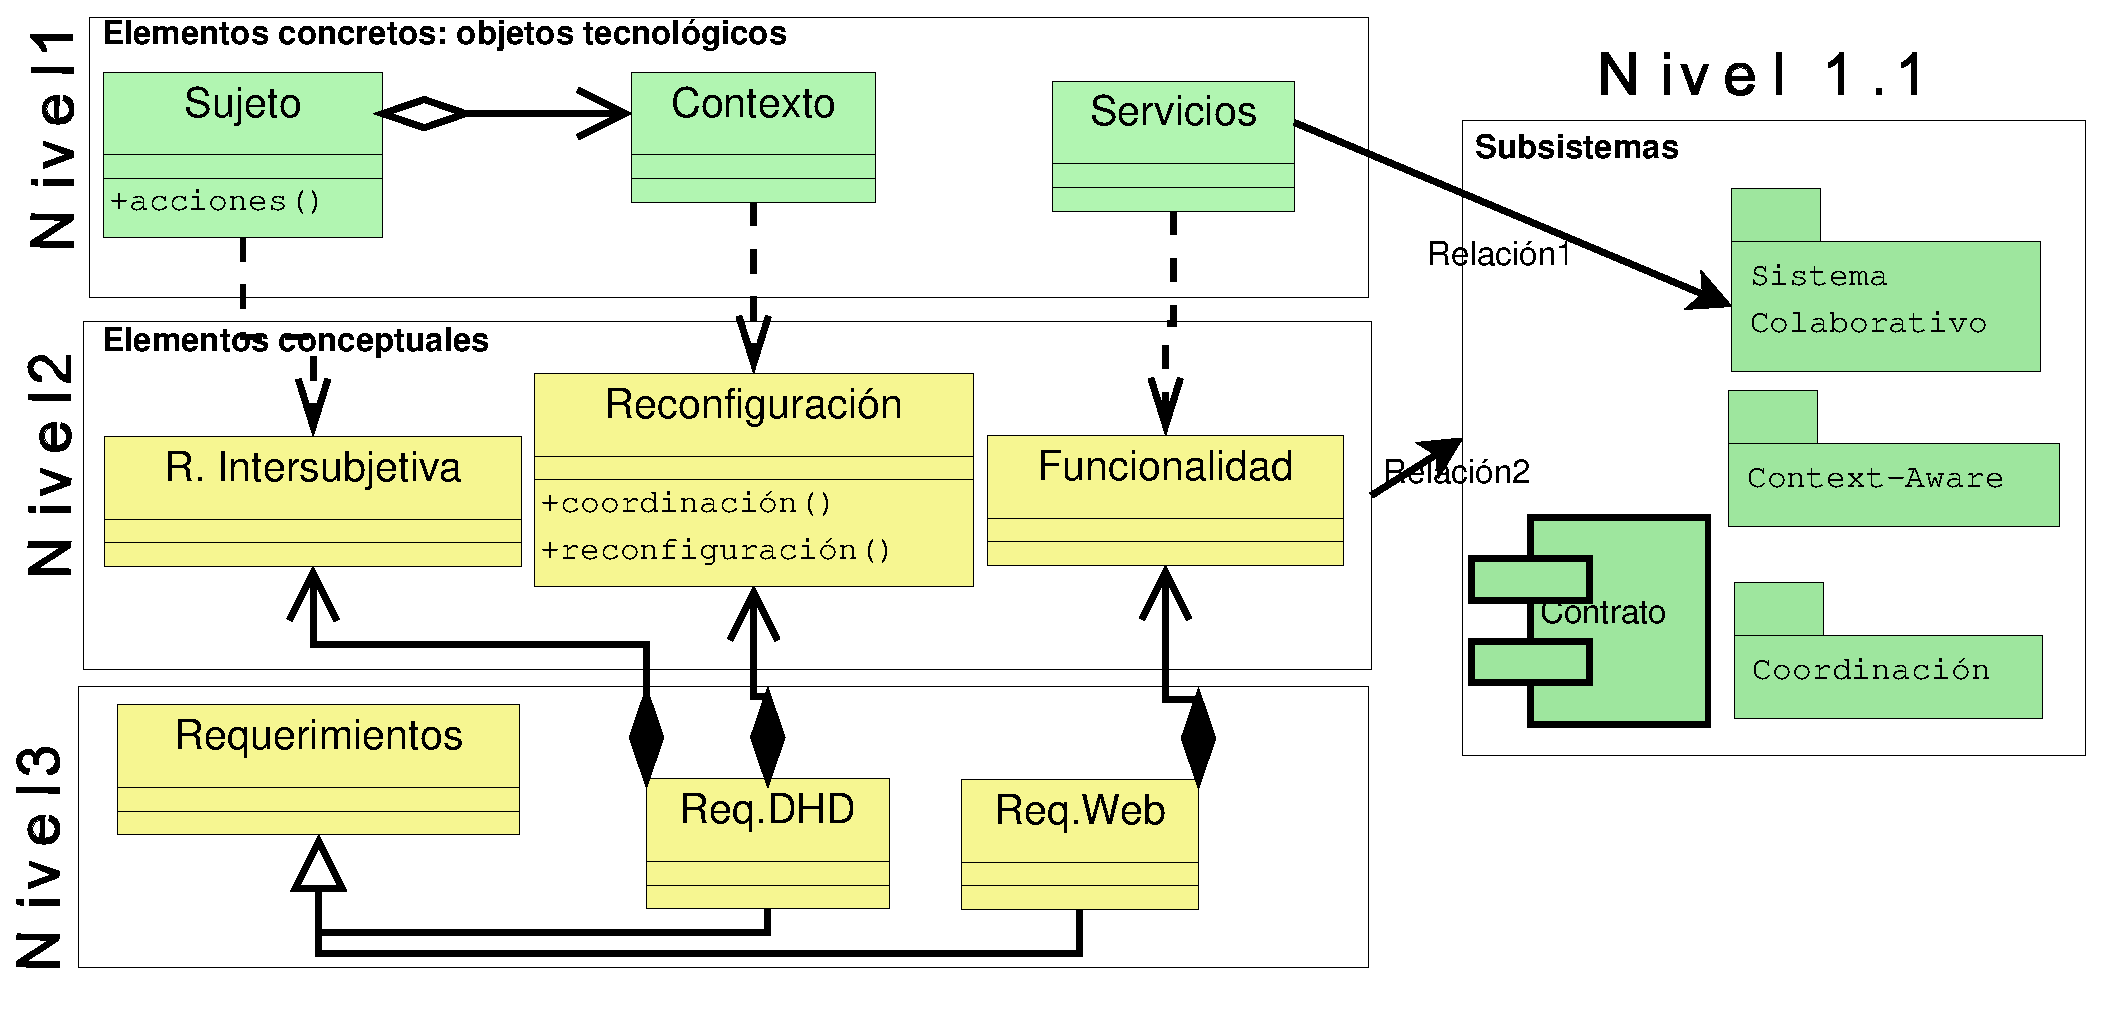
\includegraphics[width=5 in,totalheight=4 in] {DHD/RequerimientosDHD}
 % .: 0x0 pixel, 0dpi, 0.00x0.00 cm, bb=
   \caption{Niveles de abstracción y elementos de refinamientos sobre
los RequerimientosDHD} \label{fig: RequerimientosDHD}
\end{center}
\end{figure}


En el nivel 1 se encuentran las componentes tecnológicas que tienen una
influencia directa en la conformación de las componentes del nivel 2. En este
caso se representa con una flecha discontinua que las relaciones intersubjetivas
(\textit{R.Intersubjetivas}) (\ref{relaciones}) tienen una  dependencia de
concretización tecnológica desde los objetos que caracterizan a los sujetos
(\textit{Sujetos}) del DHD. De la misma manera las reconfiguración
que se producen en los DHD dependen de la posibiliad de representación y
acciones sobre el contexto. A su vez, todas las funcionalidades computables son
producto de la manipulación que se puedan lograr a partir de las
implementaciones de los servicios.  

Con el propósito de reforzar la definición de requerimientos para los DHD,
el nivel 3 se utiliza para distinguir cuales son los elementos concretos (del
nivel 2) en los cuales se basa nuestra redefinición del Dispositivo Hipermedial
Dinámico para acercarlo a la posibilidad de representaciones computacionales. 

Por otro lado, en el nivel 1.1 se encuentran los elementos que se agregan a los
del nivel 1 para aportar mejor representación, diseño e implementación de
los RequerimientosDHD. Se debe entender que en la forma en la que se relacionan
estos elementos con los anteriores establecen un modelo que fija el diseño
computacional de los DHD. Esto último ahora debe verse también como una
justificación de los argumentos expuestos en la definición del plano 3
(\ref{plano3}). Estructuralmente, dicho modelo respeta la lógica de que
indefectiblemente debe existir un nuevo nivel de representación de las
funcionalidades, requerimientos y requisitos en la construcción de DHD. Este
nivel es el que concentra el máximo trabajo multidisciplinario del grupo Obra
Abierta para la definición del DHD a partir de su conceptualización inicial.  

La figura \ref{requerimientosdhd} muestra 3 subsistemas relacionados dentro del
nivel 1.1 y una componente (\textit{Contrato}) que tendrá un protagonismo
conceptual importante en esta tesis. Las cuestiones de diseño, implementación
y uso de los subsistemas serán tratadas en los capítulos siguiente. En ellos
se verán cómo a partir de un framework colaborativo Web son utilizados sus
servicios bases (relación 1). A su vez, los elementos de reconfiguración
estarán ligado a un mecanismo de coordinación a partir de la intervención de
los contratos. Al mismo tiempo se tendrá otro subsistema encargado de la
manipulación y representación de contexto. Estos mismos elementos
intervendrán en el tratamiento de las relaciones intersubjetivas donde su
nivel de expresión quedará supeditada su forma de relacionarlos.

\begin{figure}[h]
\begin{center}
 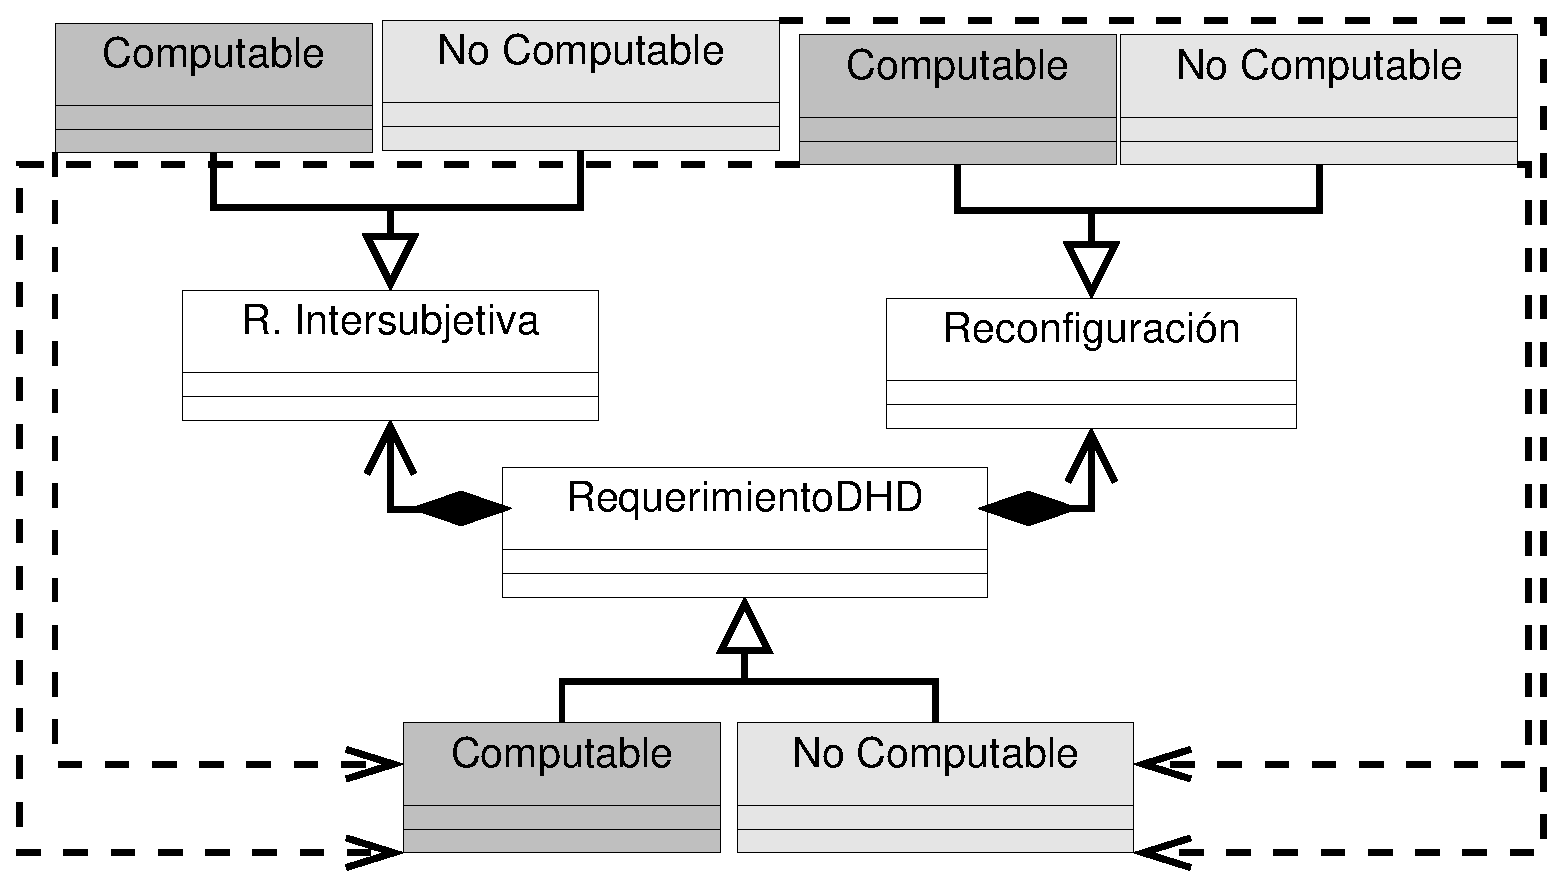
\includegraphics[width=3 in,totalheight=3 in] {DHD/RequerimientosDHD2}
 % .: 0x0 pixel, 0dpi, 0.00x0.00 cm, bb=
\caption{Estructura del RequerimientoDHD} \label{RequerimientosDHD2}
\end{center}
 \end{figure}

Ahora, estamos en condiciones de establecer una representación sobre la
estructura que determinan a los requerimientos de los DHD uniendo los conceptos
enunciados al comienzo del capítulo sobre los dos items de la sección
\ref{requerimientositems} sobre la distinción sobre el tipo de computabilidad
y no-computabilidad de los requerimientos. En la figura \ref{RequerimientosDHD2}
de los requerimientos DHD tiene que ver con computabilidad o no-computalidad que
se producen en las interacciones subjetivas (\ref{interacciones}) y
los respectivos procesos de reconfiguración. 


\section{Conclusiones}

En el comienzo del capítulo rápidamente se enuncia el rol protagónico que
tendrá la abstracción para la representación del DHD a través de elementos
tecnológicos y sus diferentes representaciones que permitan una asociación
concreta con otros tipos de elementos que se encuentran en diferentes niveles
de abstracción. De esta manera se propuso una posible
especificación sobre la naturaleza de los requerimientos de los DHD. Esta
decisión permitió una nueva definición del DHD desde la óptica de sus
requerimientos. Que a su vez permitió aplicar una teoría bien conocida para su
abordaje. Entonces, se logró identificar un patrón en el que se encuentra la
estructura de los RequerimientosDHD, lo cual facilitará su tratamiento
tecnológico. 
